\documentclass[a4paper,10pt]{article}
\usepackage[french]{babel}
\usepackage[utf8]{inputenc}
\usepackage[left=2.5cm,top=2cm,right=2.5cm,nohead,nofoot]{geometry}
\usepackage{url}
\usepackage[T1]{fontenc}
\usepackage{float}
\usepackage{afterpage}
\usepackage{amsmath}
\usepackage{amsfonts}
\usepackage{tabularx}
\usepackage{csquotes}
\usepackage{fullpage}
\usepackage{pdfpages}
\usepackage{listings}
\usepackage{color}
\usepackage{listings}
\usepackage{mdframed}
\usepackage{color}
\usepackage{pdflscape}
\usepackage{graphicx}
\graphicspath{ {images/} }

\definecolor{mygreen}{rgb}{0,0.6,0}
\definecolor{mygray}{rgb}{0.5,0.5,0.5}
\definecolor{mymauve}{rgb}{0.58,0,0.82}

\lstset{ %
  backgroundcolor=\color{white},   % choose the background color; you must add \usepackage{color} or \usepackage{xcolor}
  basicstyle=\footnotesize,        % the size of the fonts that are used for the code
  breakatwhitespace=false,         % sets if automatic breaks should only happen at whitespace
  breaklines=true,                 % sets automatic line breaking
  captionpos=b,                    % sets the caption-position to bottom
  commentstyle=\color{mygreen},    % comment style
  deletekeywords={...},            % if you want to delete keywords from the given language
  escapeinside={\%*}{*)},          % if you want to add LaTeX within your code
  extendedchars=true,              % lets you use non-ASCII characters; for 8-bits encodings only, does not work with UTF-8
  frame=single,                    % adds a frame around the code
  keepspaces=true,                 % keeps spaces in text, useful for keeping indentation of code (possibly needs columns=flexible)
  keywordstyle=\color{blue},       % keyword style
  language=Octave,                 % the language of the code
  otherkeywords={*,...},           % if you want to add more keywords to the set
  numbers=left,                    % where to put the line-numbers; possible values are (none, left, right)
  numbersep=5pt,                   % how far the line-numbers are from the code
  numberstyle=\tiny\color{mygray}, % the style that is used for the line-numbers
  rulecolor=\color{black},         % if not set, the frame-color may be changed on line-breaks within not-black text (e.g. comments (green here))
  showspaces=false,                % show spaces everywhere adding particular underscores; it overrides 'showstringspaces'
  showstringspaces=false,          % underline spaces within strings only
  showtabs=false,                  % show tabs within strings adding particular underscores
  stepnumber=2,                    % the step between two line-numbers. If it's 1, each line will be numbered
  stringstyle=\color{mymauve},     % string literal style
  tabsize=2,                     % sets default tabsize to 2 spaces
  title=\lstname                   % show the filename of files included with \lstinputlisting; also try caption instead of title
}

\usepackage[pdftex,
            pdfauthor={A. Caccia, A. Madeira Cortes},
            pdftitle={Informatique Fondamentale - Projet},
            pdfsubject={INFO-F-302 : Informatique Fondamentale - Projet}]{hyperref}

\linespread{1.1}

\setlength{\parskip}{0.5em}

\def\ojoin{\setbox0=\hbox{$\bowtie$}%
  \rule[-.02ex]{.25em}{.4pt}\llap{\rule[\ht0]{.25em}{.4pt}}}
\def\leftouterjoin{\mathbin{\ojoin\mkern-5.8mu\bowtie}}
\def\rightouterjoin{\mathbin{\bowtie\mkern-5.8mu\ojoin}}
\def\fullouterjoin{\mathbin{\ojoin\mkern-5.8mu\bowtie\mkern-5.8mu\ojoin}}

\begin{document}

\begin{titlepage}
    \begin{center}
        \textbf{\textsc{Université Libre de Bruxelles}}\\
        \textbf{\textsc{Faculté des Sciences}}\\
        \textbf{\textsc{Département d'Informatique}}

        \vfill{}
        \vfill{}

        \begin{center}
            {\Huge INFO-F-302 : Informatique Fondamentale}
        \end{center}

        {\Huge \par}

        \begin{center}
            {\LARGE Projet : Modélisation du problème du orthogonal packing et résolution avec l’outil MiniSat}
        \end{center}

        {\Huge \par}

        \begin{center}
            {\large A. Caccia, A. Madeira Cortes}
        \end{center}

        {\Huge \par}
        \vfill{}
        \vfill{}

        {\large\par}
        \vfill{}
        \vfill{}
        % \enlargethispage{3cm} % do not remove

        \textbf{Année académique 2015--2016}
    \end{center}
\end{titlepage}

\tableofcontents
\newpage

\section{Énoncé}

Soit la largeur une dimension verticale et la longueur une dimension horizontale.

Soit R un rectangle de largeur et longueur $n, m \in \mathbb{N}_{>0}$.

Soit Rec l'ensemble des k rectangles à insérer dans R, chacun plus petit que R ( $\{ r_1, r_2, \ldots r_k \}$).

Soient $\mathcal{X}$ et $\mathcal{Y}$ deux fonctions qui donnent la largeur et la longueur, respectivement, de chaque rectangle.

\section{Questions}

\subsection{Question 1: Formalisation des contraintes que doit satisfaire $\mu$}

Les contraintes sont les suivantes:

\begin{enumerate}
\item Unicité : chaque rectangle n'est utilisé qu'une seule fois
\item Existence : tous les rectangles sont ajoutés dans R
\item Chevauchement : les rectangles ne se superposent pas
\item Limites : les rectangles ne dépassent pas les bords de R
\end{enumerate}

Les traductions en langage mathématique sont les suivantes:

\textbf{Unicité}

\begin{equation}
  \label{eq:unicite1}
  \forall r_i, r_j \in Rec, \forall a \in (1..n), \forall b \in (1..m) : \mu(i) = (a, b) \land \mu(j) = (a, b) \Rightarrow i = j
\end{equation}
\begin{equation}
  \label{eq:unicite2}
  \forall r_i \in Rec, \forall a1, a2 \in (1..n), \forall b \in (1..m) : \mu(i) = (a1, b) \land \mu(i) = (a2, b) \Rightarrow a1 = a2
\end{equation}
\begin{equation}
  \label{eq:unicite3}
  \forall r_i \in Rec, \forall a \in (1..n), \forall b1, b2 \in (1..m) : \mu(i) = (a, b1) \land \mu(i) = (a, b2) \Rightarrow b1 = b2
\end{equation}

\textbf{Existence}

\begin{equation}
\label{eq:existence}
\forall r_i \in Rec : \mu(i) = (a,b)
\end{equation}

\textbf{Chevauchement}

Soit $\mu(i) = (a,b)$ et $\mu(j) = (c,d)$

\begin{equation}
\label{eq:chevauchement}
\forall r_i,r_j \in Rec : (a + \mathcal{X}(i) \leq c) \lor (c + \mathcal{X}(j) \leq a) \lor (b + \mathcal{Y}(i) \leq d) \lor (d + \mathcal{Y}(j) \leq b)
\end{equation}

\textbf{Limites}

\begin{equation}
\label{eq:limites}
\forall r_i \in Rec : (a \geq 0) \land (b \geq 0) \land (a+\mathcal{X}(i) \leq m) \land (b + \mathcal{Y}(i) \leq n)
\end{equation}

\newpage

\subsection{Question 2: Construction d'une formule en FNC telle que celle-ci est SAT ssi il existe $\mu$ correcte}

Soit prop un cube de propositions de dimensions n, m et k tel que prop(i,a,b) est vrai si le rectangle $r_i$ a pour coin inférieur gauche le point (a,b).

\textbf{Unicité}

$$C_{1.1} : \bigwedge_{\substack{0 \leq a < n \\ 0 \leq b < m}}\; \bigwedge_{\substack{1 \leq i \leq k \\ 1 \leq j \leq k \\ i \neq j}} \neg prop(i,a,b) \lor \neg prop(j,a,b)$$

$$C_{1.2} : \bigwedge_{\substack{1 \leq i \leq k \\ 0 \leq b < m}}\; \bigwedge_{\substack{0 \leq a < n \\ 0 \leq a2 < n \\ a \neq a2}} \neg prop(i,a,b) \lor \neg prop(i,a2,b)$$

$$C_{1.3} : \bigwedge_{\substack{1 \leq i \leq k \\ 0 \leq a < n}}\; \bigwedge_{\substack{0 \leq b < m \\ 0 \leq b2 < m \\ b \neq b2}} \neg prop(i,a,b) \lor \neg prop(i,a,b2)$$

\begin{center}
$$C_1: C_{1.1} \wedge C_{1.2} \wedge C_{1.3}$$
\end{center}

\textbf{Existence}

$$C_2 : \bigwedge_{\substack{1 \leq i \leq k \\ 0 \leq a < n \\ 0 \leq b < m }} prop(i,a,b) $$

\textbf{Chevauchement}

$$C_3 : \bigwedge_{\substack{1 \leq i \leq k \\ 0 \leq a < n \\ 0 \leq b < m}}\;\; \bigwedge_{\substack{0 \leq da< a + X(i) \\ 0 \leq db < b + Y(i) \\ 1 \leq i2 \leq k}} \neg prop(i,a,b) \lor \neg prop(i2,a+da,b+db)$$

\textbf{Limites}

$$C_{4.1} : \bigwedge_{1 \leq i \leq k} \;\; \bigwedge_{\substack{(n-X(i)+1) \leq a < n \\ 0 \leq b < m}} \neg prop(i,a,b)$$

$$C_{4.2} : \bigwedge_{1 \leq i \leq k} \;\; \bigwedge_{\substack{(m-Y(i)+1) \leq b < m \\ 0 \leq a < n}} \neg prop(i,a,b)$$

\begin{center}
$$C_4: C_{4.1} \wedge C_{4.2}$$
\end{center}


\begin{center}
$$FNC: C_1 \wedge C_2 \wedge C_3 \wedge C_4$$
\end{center}

\newpage

\subsection{Question 3: Implémentation et tests sur des exemples simples}

Deux fichiers reflètent l'implémentation, ``Grid.cpp'' et ``mainQ3.cpp''. Grid parse les valeurs données à la main ou via un fichier et les stocke. Le main, lui, retranscrit les contraintes en code que miniSat peut utiliser pour construire le cube de propositions évoqué plus haut, puis cherche si une solution existe. Si une solution est trouvée, il affiche le mot ``SAT'' puis des variables correspondant à une telle solution (comme décrit dans l'énoncé). Si aucune solution est trouvée, il affiche ``UNSAT''.

Pour tester le projet, il suffit de lancer les deux commandes suivantes:

\begin{lstlisting}
make Q3
cat examples/<exemple a tester>.txt | ./a.out
\end{lstlisting}

Nous avons donc testé les deux exemples donnés 
\begin{figure}[htb!]
\centering
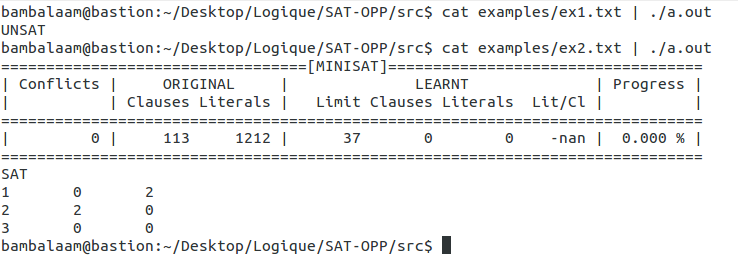
\includegraphics[scale=0.5]{SAT-Simple}
\end{figure}

Nous avons également testé un exemple plus complexe, nommé BENG06, pour lequel nous avons obtenu une réponse (affichée ici tronquée car la réponse comporte 40 lignes de données affichées).

\begin{figure}[htb!]
\centering
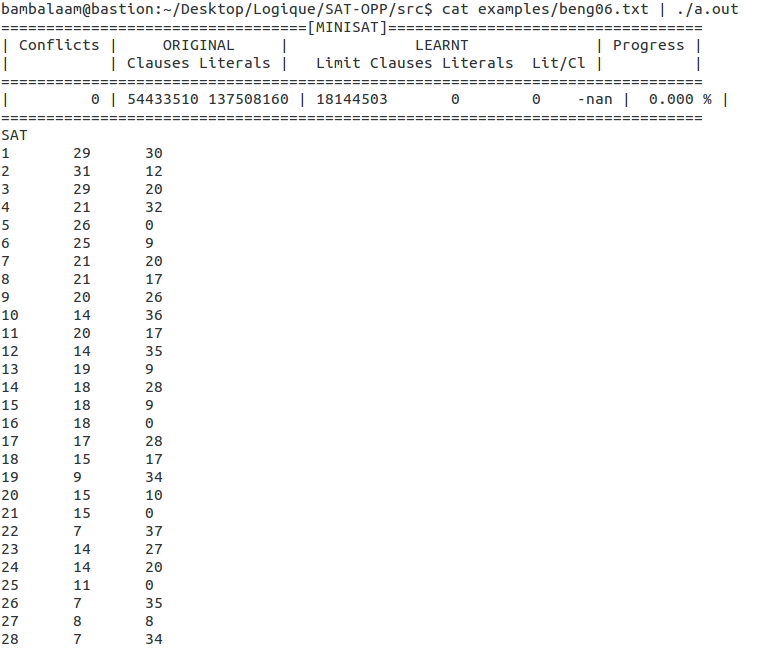
\includegraphics[scale=0.45]{SAT-BENG06}
\end{figure}

\newpage

\subsection{Question 4: Si R est un carré, trouver la plus petite dimension de celui-ci admettant une solution pour des rectangles donnés}

Soit R de dimensions $s \times s$.

On incrémente depuis un s minimum qui est la plus grande largeur ou longueur du plus grand rectangle, jusqu'à trouver une solution valable.

Une amélioration possible serait d'effectuer une recherche dichotomique entre ce s minimum et le s maximal possible qui serait la plus grande taille de tous les rectangles mis bout à bout sur la largeur ou longueur.

La question 5 étant une variante de la 4 seulement dans le format de l'input, nous présentons qu'un seul exemple pour les deux, à voir dans la sous-section suivante.

\subsection{Question 5: Si R est un carré et n un entier donné, trouver la plus petite dimension de R admettant une solution pour des carrés de taille $i \times i$ pour tout $i \leq n$}

Même chose que pour la question 4, mais avec création des carrés à insérer de tailles contenues entre 1 et n.

Pour le lancer, il suffit de lancer les commandes suivantes
\begin{lstlisting}
make Q5
./a.out
\end{lstlisting}

Le programme vous demandera d'entrer un nombre à tester.

Voici donc un exemple de solution:

\begin{figure}[htb!]
\centering
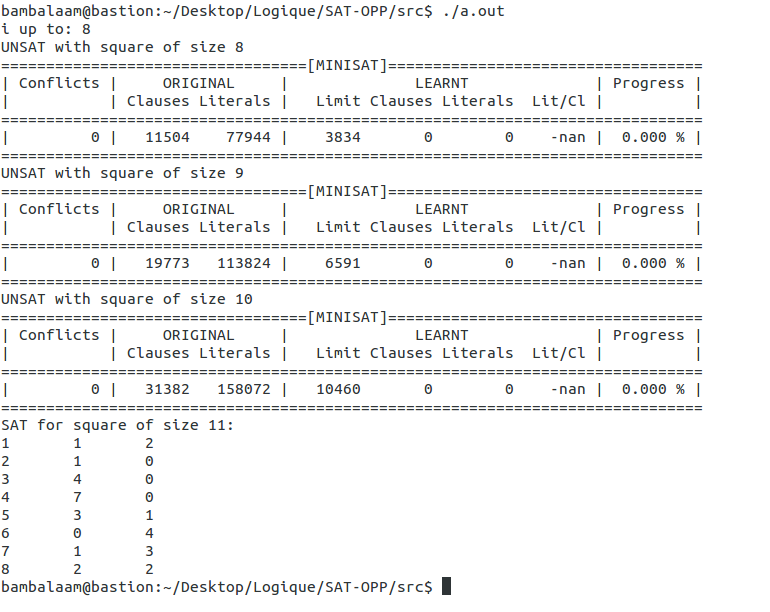
\includegraphics[scale=0.50]{SAT-Q5}
\end{figure}

\newpage

\subsection{Question 6: Ajout d'une troisième dimension}

Les contraintes n'ont pas changé dans le fond, elles reflètent simplement l'ajout d'une dimension en plus.

Pour le lancer, même chose que pour la question 3, mais avec ``make Q6'' à la place. Bien sur, les fichiers à utiliser sont également différents puisque une dimension en plus doit être présente. Voici un screenshot du lancement de la résolution de cette question sur des variantes des exemples disponibles dans l'énoncé auxquels nous avons juste rajouté la troisième dimension.

\begin{figure}[htb!]
\centering
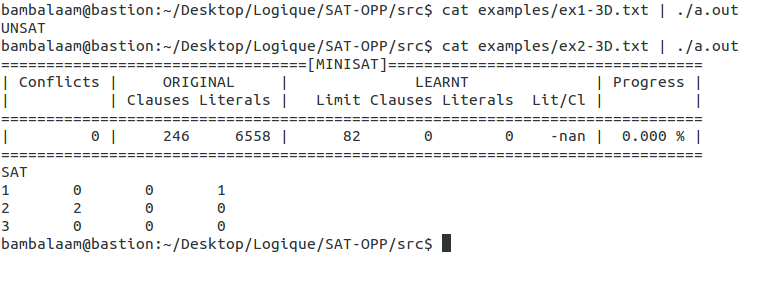
\includegraphics[scale=0.50]{SAT-3D}
\end{figure}

\subsection{Question 7: Contrainte - ne pas faire flotter des pavés droits dans l'espace}

Vu que cela n'était pas défini dans l'énoncé, nous avons assumé que la base d'un pavé droit W posé sur un pavé droit V doit être contenu sur le sommet du pavé droit V. C'est à dire, graphiquement, si l'on imagine des pavés droits vu de coté:

\begin{figure}[htb!]
\centering
\includegraphics[scale=0.8]{possible}
\end{figure}

Nous avons décidé de le définir comme ceci car, d'un point de vue réaliste, il est possible qu'un pavé droit posé sur un autre le dépasse légèrement niveau taille, mais à partir de quand est-ce que l'on considère qu'il est ``trop'' grand et flotte/tombe?

Donc, formellement:

Soit $\mu(v) = (a,b,c)$ et $\mu(w) = (d,e,f)$

$(f = c + \mathcal{Z}(v)) \land (d \geq a) \land (d+\mathcal{X}(w) \leq a+\mathcal{X}(v)) \land (e \geq b) \land(e+\mathcal{Y}(w) \leq b+\mathcal{Y}(v))$

\section{Conclusion}

Nous avons trouvé ce projet fort intéressant (vraiment, c'est pas une blague), mais malheureusement, vu le nombre assez conséquent de projets à rendre nous n'avons pas pu y consacrer le temps qu'il serait requis pour nous lancer dans les questions bonus. Néanmoins, le plaisir de voir le projet fonctionner pour des exemples plus complexes a été le point fort de cette semaine chargée en travail et rebondissements.

\end{document}
